
\chapter{Diage modelling language}
In this chapter I will cover the Diage Modelling Language (DML) that is used to visualize the flow of information, some are static and others will wait for the interaction of the player to release this information and ensuring plot progression. \diage uses the symbols to represent the \diage entities as seen in figure~\ref{fig:DMLSymbols}. 

\begin{figure}[h]
	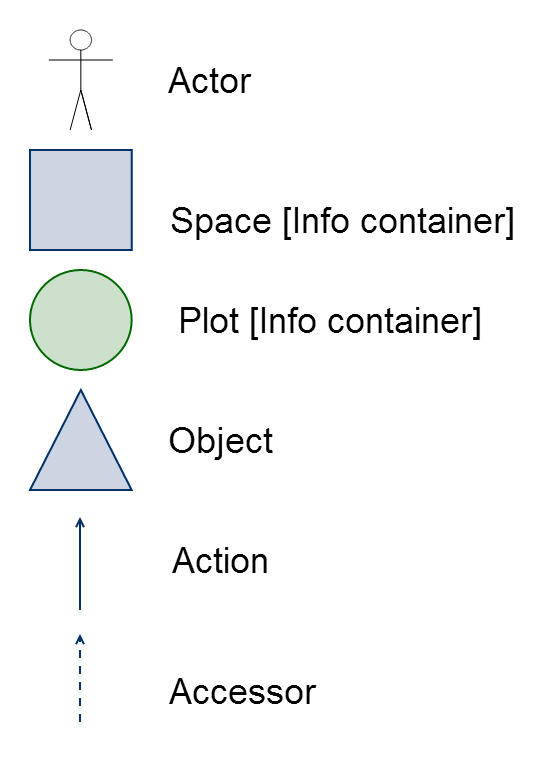
\includegraphics[scale=.3]{symbols}
	\caption{DML Symbols}
	\label{fig:DMLSymbols}	
\end{figure}

\section{Actors}
An actor is the representation of any one object that can, as the noun implies, act. Examples are the store-clerk, a wandering adventurer or the player. The actor is the only entity that can physically interact with the world, and by doing so changing the world's state. By being able to change the world, the actors are the only entities that can ensure plot progression. An actor has two properties; \code{name} and \code{type}. The type property is used in predefined actions as seen in figure~\ref{fig:actions:npc}. This defines that the \code{Player} can speak to all actors of type \code{NPC}\footnote{This can be generalized for all entities, I guess.}. 


\begin{figure}[ht]
	\centering
	\begin{subfigure}[b]{0.3\textwidth}
		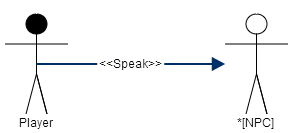
\includegraphics[width=\textwidth]{npc_action}
		\caption{A standard action for NPC interaction}\label{fig:actions:npc}
	\end{subfigure}
	\begin{subfigure}[b]{0.3\textwidth}
		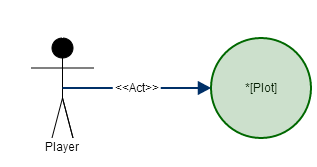
\includegraphics[width=\textwidth]{plot_action}
		\caption{A standard action for plot interaction}\label{fig:actions:plot}
	\end{subfigure}
	\begin{subfigure}[b]{0.3\textwidth}
		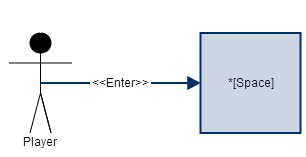
\includegraphics[width=\textwidth]{space_action}
		\caption{A standard action for space interaction}\label{fig:actions:space}
	\end{subfigure}
	\caption{Predefined actions}\label{fig:actions}
\end{figure}

\begin{figure}[ht]
	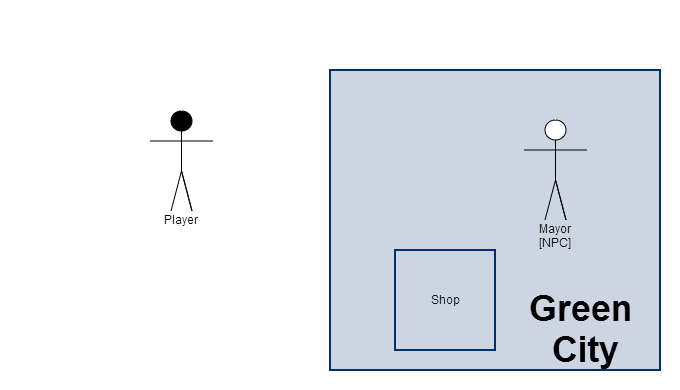
\includegraphics[scale=.5]{diagram_actor_example}
	\caption{An example of a Diage diagram using predefined actions}\label{fig:examplediagram}
\end{figure}



\begin{figure}
	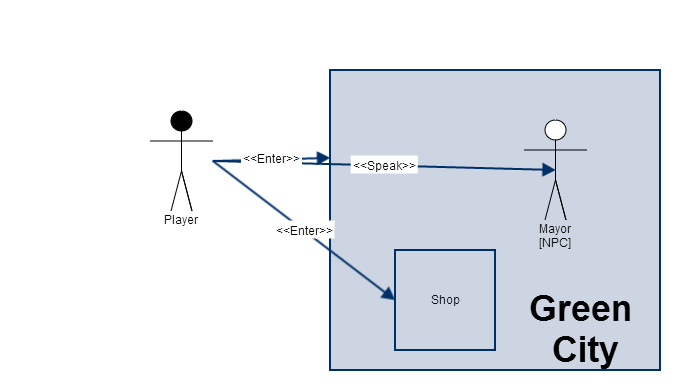
\includegraphics[scale=.5]{diagram_actor_example_verbose}
	\caption{An example of a Diage diagram without using predefined actions}\label{fig:examplediagramverbose}
\end{figure}